In diesem Kapitel werden alle Grundlagen erläutert, welche nötig sind um den Versuch durchführen zu können. 
\subsection{Die Lichtgeschwindkeit heute}
An der Internationalen Konferenz für Mass und Gewicht kurz ICPM wurde der Meter durch Festlegung des Zahlenwertes für die Lichgeschwindigkeit im Vakuum wie folgt neu definiert.

%%%%%%%%%%%%%%%%%%%%%%%%%%%%%%%%%%%%%%%%%%%%%%%%%%%%%%%%%%%%%%%%%%%%%%%%%%%%%
\begin{equation*}
c_{0} = 299'792'458 m/s
\label{eq:Lichtgeschwindigkeit}
\end{equation*}
%%%%%%%%%%%%%%%%%%%%%%%%%%%%%%%%%%%%%%%%%%%%%%%%%%%%%%%%%%%%%%%%%%%%%%%%%%%%%

Die Lichtgeschwindigkeit in einem Medium wiederrum erhält man mit Hilfe des gemessenen Brechungsindexes $c=c_{0}/n$. In einem Gas, also zum Beispiel in der Luft, ist n proportional zur Dichte und wird noch durch die Luftfeuchtigkeit leicht beeinflusst.


%%%%%%%%%%%%%%%%%%%%%%%%%%%%%%%%%%%%%%%%%%%%%%%%%%%%%%%%%%%%%%%%%%%%%%%%%%%%%
\begin{equation}
(n - 1) = (n_{n} - 1)\cdot\dfrac{p \cdot T_{n}}{p_{n} \cdot T}-(\beta - \dfrac{\gamma}{\gamma}_{0}) \cdot p_{w}
\label{eq:Lichtgeschwindigkeit}
\end{equation}
%%%%%%%%%%%%%%%%%%%%%%%%%%%%%%%%%%%%%%%%%%%%%%%%%%%%%%%%%%%%%%%%%%%%%%%%%%%%%

%%%%%%%%%%%%%%%%%%%%%%%%%%%%%%%%%%%%%%%%%%%%%%%%%%%%%%%%%%%%%%%%%%%%%%%%%%%%%
\begin{figure}[htb]
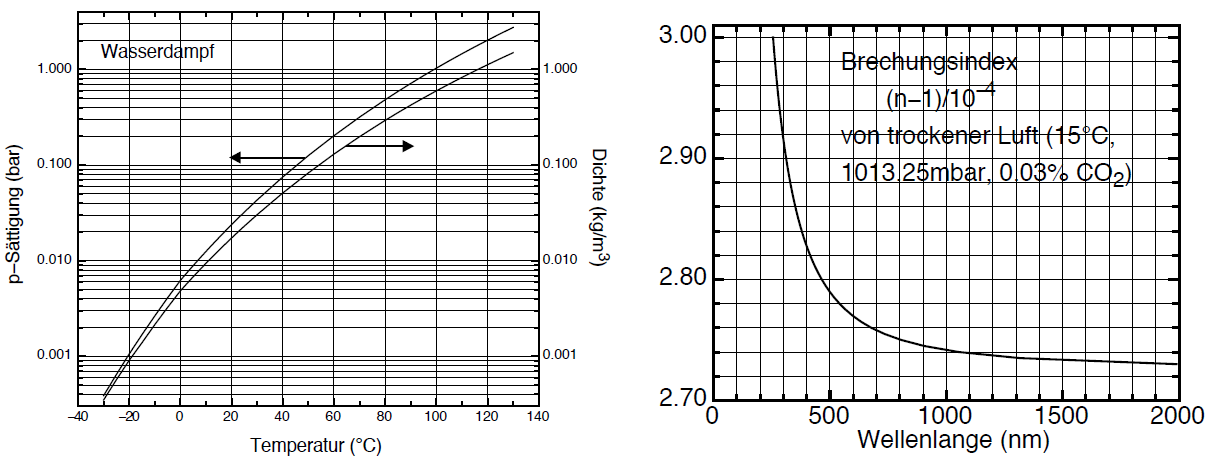
\includegraphics[width=\textwidth]{Brechungsindex_Luft_Grafik.png}
\caption{Wasserdampfsättigung und Normbrechungsindex}
\label{fig:Wasserdampfsättigung und Normbrechungsindex}
\end{figure}
%%%%%%%%%%%%%%%%%%%%%%%%%%%%%%%%%%%%%%%%%%%%%%%%%%%%%%%%%%%%%%%%%%%%%%%%%%%%%

\subsection{Messung der Lichtgeschwindigkeit nach Michelson}
